\begin{minipage}{.5\textwidth}
\begin{tikzpicture}
  \begin{axis}[
    title={Test stacked},
    xbar stacked, xmin=0,  
    bar width=10mm,
    symbolic y coords={Instrument},
    ytick=data,
    nodes near coords, 
    nodes near coords align={anchor=north},%Move values in bar
    every node near coord/.style={
    },
  ]
  %Active
  \addplot [fill=green] coordinates {
({Instrument},15)};
  %Inactive
  \addplot [fill=red] coordinates {
({Instrument},60)};
  \legend{Active,Inactive}
  \end{axis}
 \end{tikzpicture}
 \end{minipage}
 \hspace{2.5cm}
\begin{minipage}{.5\textwidth}
 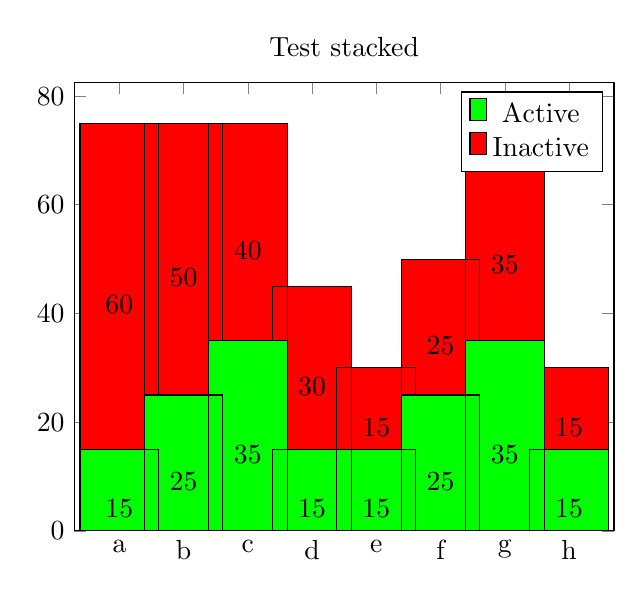
\begin{tikzpicture}
  \begin{axis}[
    title={Test stacked},
    ybar stacked, ymin=0,  
    bar width=10mm,
    symbolic x coords={a,b,c,d,e,f,g,h},
    xtick=data,
    nodes near coords, 
    nodes near coords align={anchor=north},%Move values in bar
    every node near coord/.style={
    },
  ]
  %Active
  \addplot [fill=green] coordinates {
({a},15)
({b},25)
({c},35)
({d},15)
({e},15)
({f},25)
({g},35)
({h},15)};
  %Inactive
  \addplot [fill=red] coordinates {
({a},60)
({b},50)
({c},40)
({d},30)
({e},15)
({f},25)
({g},35)
({h},15)};
  \legend{Active,Inactive}
  \end{axis}
 \end{tikzpicture}
 \end{minipage}

